% Options for packages loaded elsewhere
\PassOptionsToPackage{unicode}{hyperref}
\PassOptionsToPackage{hyphens}{url}
\PassOptionsToPackage{dvipsnames,svgnames*,x11names*}{xcolor}
%
\documentclass[
  10pt,
]{article}
\usepackage{lmodern}
\usepackage{setspace}
\usepackage{amssymb,amsmath}
\usepackage{ifxetex,ifluatex}
\ifnum 0\ifxetex 1\fi\ifluatex 1\fi=0 % if pdftex
  \usepackage[T1]{fontenc}
  \usepackage[utf8]{inputenc}
  \usepackage{textcomp} % provide euro and other symbols
\else % if luatex or xetex
  \usepackage{unicode-math}
  \defaultfontfeatures{Scale=MatchLowercase}
  \defaultfontfeatures[\rmfamily]{Ligatures=TeX,Scale=1}
  \setmainfont[]{DejaVu Serif}
  \setmonofont[]{DejaVu Sans Mono}
\fi
% Use upquote if available, for straight quotes in verbatim environments
\IfFileExists{upquote.sty}{\usepackage{upquote}}{}
\IfFileExists{microtype.sty}{% use microtype if available
  \usepackage[]{microtype}
  \UseMicrotypeSet[protrusion]{basicmath} % disable protrusion for tt fonts
}{}
\makeatletter
\@ifundefined{KOMAClassName}{% if non-KOMA class
  \IfFileExists{parskip.sty}{%
    \usepackage{parskip}
  }{% else
    \setlength{\parindent}{0pt}
    \setlength{\parskip}{6pt plus 2pt minus 1pt}}
}{% if KOMA class
  \KOMAoptions{parskip=half}}
\makeatother
\usepackage{xcolor}
\IfFileExists{xurl.sty}{\usepackage{xurl}}{} % add URL line breaks if available
\IfFileExists{bookmark.sty}{\usepackage{bookmark}}{\usepackage{hyperref}}
\hypersetup{
  colorlinks=true,
  linkcolor=red,
  filecolor=red,
  citecolor=red,
  urlcolor=red,
  pdfcreator={LaTeX via pandoc}}
\urlstyle{same} % disable monospaced font for URLs
\usepackage[margin=1cm,top=1cm,bottom=1cm,left=1cm,right=1cm,includeheadfoot]{geometry}
\usepackage{listings}
\newcommand{\passthrough}[1]{#1}
\lstset{defaultdialect=[5.3]Lua}
\lstset{defaultdialect=[x86masm]Assembler}
\usepackage{graphicx}
\makeatletter
\def\maxwidth{\ifdim\Gin@nat@width>\linewidth\linewidth\else\Gin@nat@width\fi}
\def\maxheight{\ifdim\Gin@nat@height>\textheight\textheight\else\Gin@nat@height\fi}
\makeatother
% Scale images if necessary, so that they will not overflow the page
% margins by default, and it is still possible to overwrite the defaults
% using explicit options in \includegraphics[width, height, ...]{}
\setkeys{Gin}{width=\maxwidth,height=\maxheight,keepaspectratio}
% Set default figure placement to htbp
\makeatletter
\def\fps@figure{htbp}
\makeatother
\setlength{\emergencystretch}{3em} % prevent overfull lines
\providecommand{\tightlist}{%
  \setlength{\itemsep}{0pt}\setlength{\parskip}{0pt}}
\setcounter{secnumdepth}{3}
% Enable graphics inclusion and ensure figure numbering works
\usepackage{graphicx}
\renewcommand{\figurename}{Figure}

% Configure fonts for Unicode support with fallbacks
\usepackage{newunicodechar}
\newunicodechar{⁴}{\textsuperscript{4}}
\newunicodechar{₄}{\textsubscript{4}}

% Enhanced code block styling for better contrast and readability
\usepackage{fancyvrb}
\usepackage{xcolor}
\usepackage{listings}

% Define custom colors for code blocks
\definecolor{codebg}{RGB}{245, 245, 245}      % Light gray background
\definecolor{codeborder}{RGB}{200, 200, 200}  % Medium gray border
\definecolor{codefg}{RGB}{50, 50, 50}         % Dark gray text

% Configure Verbatim environment for inline code
\DefineVerbatimEnvironment{Verbatim}{Verbatim}{%
    fontsize=\small,
    frame=single,
    framerule=0.5pt,
    framesep=3pt,
    rulecolor=\color{codeborder},
    bgcolor=\color{codebg},
    fgcolor=\color{codefg}
}

% Configure code block styling
\DefineVerbatimEnvironment{Highlighting}{Verbatim}{%
    fontsize=\footnotesize,
    frame=single,
    framerule=0.5pt,
    framesep=5pt,
    rulecolor=\color{codeborder},
    bgcolor=\color{codebg},
    fgcolor=\color{codefg}
}

% Style inline code with \texttt
\renewcommand{\texttt}[1]{%
    \colorbox{codebg}{\color{codefg}\ttfamily #1}%
}

% Configure listings package for code blocks
\lstset{
    backgroundcolor=\color{codebg},
    basicstyle=\footnotesize\ttfamily\color{codefg},
    breakatwhitespace=false,
    breaklines=true,
    captionpos=b,
    commentstyle=\color{codefg},
    deletekeywords={...},
    escapeinside={\%*}{*)},
    extendedchars=true,
    frame=single,
    framerule=0.5pt,
    framesep=5pt,
    keepspaces=true,
    keywordstyle=\color{codefg},
    language=Python,
    morekeywords={*,...},
    numbers=left,
    numbersep=5pt,
    numberstyle=\tiny\color{codefg},
    rulecolor=\color{codeborder},
    showspaces=false,
    showstringspaces=false,
    showtabs=false,
    stepnumber=1,
    stringstyle=\color{codefg},
    tabsize=2,
    title=\lstname
}

% Override any Pandoc default lstset configurations
\AtBeginDocument{
    \lstset{
        backgroundcolor=\color{codebg},
        basicstyle=\footnotesize\ttfamily\color{codefg},
        frame=single,
        framerule=0.5pt,
        framesep=5pt,
        rulecolor=\color{codeborder},
        numbers=left,
        numbersep=5pt,
        numberstyle=\tiny\color{codefg}
    }
}

% Configure hyperref colors consistently
\AtBeginDocument{
% Override pandoc's hidelinks setting with consistent options
\hypersetup{
    colorlinks=true,
    allcolors=red,
    linkcolor=red,
    urlcolor=red,
    citecolor=red,
    filecolor=red,
    menucolor=red,
    linktoc=all
}
}

\title{Optimization in 4D}
\author{Daniel Ari Friedman\\ ORCID: 0000-0001-6232-9096\\ Email: daniel@activeinference.institute}
\date{August 15, 2025}

\begin{document}
\maketitle

{
\hypersetup{linkcolor=black}
\setcounter{tocdepth}{3}
\tableofcontents
}
\setstretch{1.0}
\hypertarget{optimization-in-4d}{%
\section{Optimization in 4D}\label{optimization-in-4d}}

\hypertarget{overview}{%
\subsection{Overview}\label{overview}}

This section describes optimization methods adapted to the integer
Quadray lattice, emphasizing discrete convergence and
information-geometric approaches. The methods leverage the IVM's natural
quantization and extend to higher-dimensional spaces via Coxeter.4D
embeddings.

\hypertarget{neldermead-on-integer-lattice}{%
\subsection{Nelder--Mead on Integer
Lattice}\label{neldermead-on-integer-lattice}}

\begin{itemize}
\tightlist
\item
  \textbf{Adaptation}: standard Nelder--Mead simplex operations with
  projection to integer Quadray coordinates.
\item
  \textbf{Projection}: after each reflection/expansion/contraction, snap
  to nearest integer lattice point via projective normalization.
\item
  \textbf{Volume tracking}: monitor integer tetravolume as convergence
  diagnostic; discrete steps create stable plateaus.
\end{itemize}

\hypertarget{parameters}{%
\subsubsection{Parameters}\label{parameters}}

\begin{itemize}
\tightlist
\item
  \textbf{Reflection} \(\alpha \approx 1\)
\item
  \textbf{Expansion} \(\gamma \approx 2\)
\item
  \textbf{Contraction} \(\rho \approx 0.5\)
\item
  \textbf{Shrink} \(\sigma \approx 0.5\)
\end{itemize}

References: original Nelder--Mead method and common parameterizations in
optimization texts and survey articles; see overview:
\href{https://en.wikipedia.org/wiki/Nelder\%E2\%80\%93Mead_method}{Nelder--Mead
method}.

\hypertarget{volume-level-dynamics}{%
\subsection{Volume-Level Dynamics}\label{volume-level-dynamics}}

\begin{itemize}
\tightlist
\item
  Simplex volume decreases in discrete integer steps, creating stable
  plateaus (``energy levels'').
\item
  Termination: when volume stabilizes at a minimal level and function
  spread is below tolerance.
\item
  Monitoring: track integer simplex volume and the objective spread at
  each iteration for convergence diagnostics.
\end{itemize}

\hypertarget{pseudocode-sketch}{%
\subsection{Pseudocode (Sketch)}\label{pseudocode-sketch}}

\begin{lstlisting}
while not converged:
  order vertices by objective
  centroid of best three
  propose reflected (then possibly expanded/contracted) point
  project to integer quadray; renormalize with (k,k,k,k)
  accept per standard tests; else shrink toward best
  update integer volume and function spread trackers
\end{lstlisting}

\hypertarget{figures}{%
\subsubsection{Figures}\label{figures}}

\begin{figure}
\centering
\includegraphics{../output/figures/simplex_trace.png}
\caption{\textbf{Figure 7: Discrete Nelder--Mead optimization trajectory
on the integer Quadray lattice}. This time-series plot tracks key
diagnostic quantities across 12 optimization iterations for a simple
quadratic objective \(f(q) = (q.a - 1)^2 + q.b^2 + q.c^2 + q.d^2\)
starting from initial simplex vertices
\(\{(5,0,0,0), (4,1,0,0), (0,4,1,0), (1,1,1,0)\}\). \textbf{Left y-axis
(objective values)}: Blue line shows the best (minimum) objective value
per iteration, demonstrating monotonic improvement as the simplex
converges toward the minimum at \((1,0,0,0)\). Orange line shows the
worst (maximum) objective value among the four simplex vertices.
\textbf{Right y-axis (simplex volume)}: Green line tracks the integer
tetravolume of the current simplex computed via Tom Ace's 5×5
determinant, showing characteristic discrete plateaus and step-wise
reductions as the simplex contracts on the lattice. \textbf{Convergence
signature}: The volume decreases in discrete integer steps, creating
stable ``energy levels'' that regularize the optimization process, while
the objective spread (difference between best and worst) narrows as
vertices cluster near the optimum. The full 3D simplex trajectory
animation is available as
\passthrough{\lstinline!simplex\_animation.mp4!} in the output
directory.}
\end{figure}

\begin{figure}
\centering
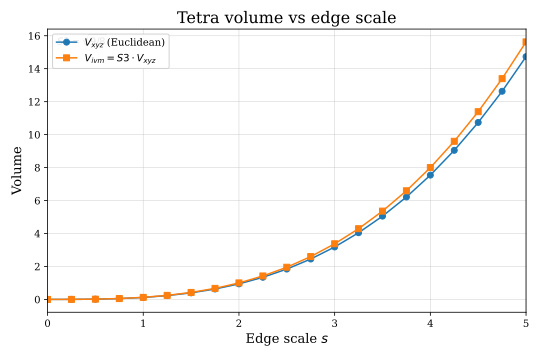
\includegraphics{../output/figures/volumes_scale_plot.png}
\caption{\textbf{Figure 8: Tetrahedron volume scaling relationships:
Euclidean vs IVM unit conventions}. This plot demonstrates the
mathematical relationship between edge length scaling and tetravolume
under both Euclidean (Coxeter.4D) and synergetics (Fuller.4D) unit
conventions. \textbf{X-axis}: Edge scale factor ranging from 0.5 to 2.0
applied to a regular tetrahedron. \textbf{Y-axis}: Computed tetravolume
in respective units. \textbf{Blue curve} (\(V_{xyz}\)): Euclidean
tetravolume computed via standard geometric formulas, showing the
expected cubic scaling relationship \(V \propto \text{edge}^3\).
\textbf{Orange curve} (\(V_{ivm}\)): IVM tetravolume obtained by
converting the Euclidean volume via the synergetics factor
\(S3 = \sqrt{9/8} \approx 1.061\), following the relationship
\(V_{ivm} = S3 \cdot V_{xyz}\). \textbf{Scaling verification}: Both
curves maintain their proportional relationship across all scales,
confirming the consistency of the S3 conversion factor used throughout
the manuscript to bridge between Coxeter.4D (Euclidean) and Fuller.4D
(IVM) volume measurements. The parallel cubic curves validate the unit
conversion methods employed in bridging vs native tetravolume
comparisons. Raw numerical data available as
\passthrough{\lstinline!volumes\_scale\_data.csv!} and
\passthrough{\lstinline!volumes\_scale\_data.npz!}.}
\end{figure}

As shown in Figure 9, the discrete Nelder--Mead converges on plateaus;
Figure 8 summarizes the scaling behavior used in volume diagnostics.

\begin{figure}
\centering
\includegraphics{../output/figures/simplex_final.png}
\caption{\textbf{Figure 9: Final converged simplex configuration in 3D
embedding space}. This 3D scatter plot shows the four vertices of the
Nelder--Mead simplex after 12 iterations of discrete optimization on the
integer Quadray lattice, projected into Euclidean 3D space via the
default embedding matrix. The green points represent the converged
simplex vertices clustered near the objective minimum, connected by
green lines to emphasize the tetrahedral structure. All vertices are
constrained to integer Quadray coordinates and maintain the projective
normalization (at least one zero component). The tight clustering
demonstrates successful convergence while the discrete lattice
constraint ensures numerical stability. This static view complements the
dynamic trajectory shown in the full animation
(\passthrough{\lstinline!simplex\_animation.mp4!}) and the diagnostic
traces in Figure 7. The final simplex volume is minimal on the integer
lattice, representing a stable ``energy level'' where further discrete
moves do not improve the objective function.}
\end{figure}

Raw artifacts: the full trajectory animation
\passthrough{\lstinline!simplex\_animation.mp4!} and per-frame vertices
(\passthrough{\lstinline!simplex\_animation\_vertices.csv!}/\passthrough{\lstinline!.npz!})
are available in \passthrough{\lstinline!quadmath/output/!}. The full
optimization trajectory is provided as an animation (MP4) in the
repository's output directory.

\hypertarget{discrete-lattice-descent-information-theoretic-variant}{%
\subsection{Discrete Lattice Descent (Information-Theoretic
Variant)}\label{discrete-lattice-descent-information-theoretic-variant}}

\begin{itemize}
\tightlist
\item
  Integer-valued descent over the IVM using the 12 neighbor moves
  (permutations of \{2,1,1,0\}), snapping to the canonical
  representative via projective normalization.
\item
  Objective can be geometric (e.g., Euclidean in an embedding) or
  information-theoretic (e.g., local free-energy proxy); monotone
  decrease is guaranteed by greedy selection.
\item
  API: \passthrough{\lstinline!discrete\_ivm\_descent!} in
  \passthrough{\lstinline!src/discrete\_variational.py!}. Animation
  helper: \passthrough{\lstinline!animate\_discrete\_path!} in
  \passthrough{\lstinline!src/visualize.py!}.
\end{itemize}

Short snippet (paper reproducibility):

\begin{lstlisting}[language=Python]
from quadray import Quadray, DEFAULT_EMBEDDING, to_xyz
from discrete_variational import discrete_ivm_descent
from visualize import animate_discrete_path

def f(q: Quadray) -> float:
    x, y, z = to_xyz(q, DEFAULT_EMBEDDING)
    return (x - 0.5)**2 + (y + 0.2)**2 + (z - 0.1)**2

path = discrete_ivm_descent(f, Quadray(6,0,0,0))
animate_discrete_path(path)
\end{lstlisting}

\hypertarget{convergence-and-robustness}{%
\subsection{Convergence and
Robustness}\label{convergence-and-robustness}}

\begin{itemize}
\tightlist
\item
  Discrete steps reduce numerical drift; improved stability
  vs.~unconstrained Cartesian.
\item
  Natural regularization from volume quantization; fewer wasted
  evaluations.
\item
  Compatible with Gauss--Newton/Natural Gradient guidance using FIM for
  metric-aware steps (Amari, natural gradient).
\end{itemize}

\hypertarget{information-geometric-view-einstein.4d-analogy-in-metric-form}{%
\subsection{Information-Geometric View (Einstein.4D analogy in metric
form)}\label{information-geometric-view-einstein.4d-analogy-in-metric-form}}

\begin{itemize}
\tightlist
\item
  \textbf{Fisher Information as metric}: use the empirical estimator
  \passthrough{\lstinline!F = (1/N) \\sum g g^\\top!} from
  \passthrough{\lstinline!fisher\_information\_matrix!} to analyze
  curvature of the objective with respect to parameters. See
  \href{https://en.wikipedia.org/wiki/Fisher_information}{Fisher
  information}.
\item
  \textbf{Curvature directions}: leading eigenvalues/eigenvectors of
  \passthrough{\lstinline!F!} (see
  \passthrough{\lstinline!fim\_eigenspectrum!}) reveal stiff and sloppy
  directions; this supports step-size selection and preconditioning.
\item
  \textbf{Figures}: empirical FIM heatmap (Figure 10) and eigenspectrum
  (Figure 11). Raw data available as NPZ/CSV in
  \passthrough{\lstinline!quadmath/output/!}.
\end{itemize}

\begin{figure}
\centering
\includegraphics{../output/figures/fisher_information_matrix.png}
\caption{\textbf{Figure 10: Empirical Fisher Information Matrix (FIM)
for noisy linear regression}. This heatmap visualizes the 3×3 Fisher
information matrix \(F_{ij}\) estimated from per-sample gradients of a
misspecified linear regression model. \textbf{Setup}: Ground truth
parameters \(w_{\text{true}} = [1.0, -2.0, 0.5]\), evaluated at
estimation point \(w_{\text{est}} = [0.3, -1.2, 0.0]\), with 200 samples
and Gaussian noise (σ=0.1). \textbf{Matrix elements}: Each \(F_{ij}\)
entry represents the expected outer product
\(\mathbb{E}[\partial_i \log p \cdot \partial_j \log p]\) where
gradients are computed from squared loss with respect to model
parameters. \textbf{Interpretation}: The colorbar scale shows local
curvature magnitudes---brighter entries indicate directions of higher
sensitivity/information content. Diagonal dominance suggests the
parameters are approximately decoupled at this evaluation point.
\textbf{Information geometry}: This FIM serves as a Riemannian metric
tensor for natural gradient descent (see Eq. \eqref{eq:supp_natgrad} in
the equations appendix), enabling curvature-aware optimization steps
that adapt to the local geometry of the parameter manifold. Raw matrix
data saved as \passthrough{\lstinline!fisher\_information\_matrix.csv!}
and \passthrough{\lstinline!fisher\_information\_matrix.npz!} for
reproducibility.}
\end{figure}

\begin{figure}
\centering
\includegraphics{../output/figures/fisher_information_eigenspectrum.png}
\caption{\textbf{Figure 11: Fisher Information Matrix eigenspectrum:
principal curvature directions}. This bar chart displays the eigenvalue
decomposition of the empirical Fisher information matrix from Figure 10,
revealing the principal curvature directions of the parameter manifold.
\textbf{X-axis}: Eigenvalue indices (0, 1, 2) sorted in descending order
of magnitude. \textbf{Y-axis}: Eigenvalue magnitudes representing the
curvature strength along corresponding eigenvector directions.
\textbf{Interpretation}: Large eigenvalues indicate ``stiff'' parameter
directions where small changes significantly affect the objective
function, while small eigenvalues correspond to ``sloppy'' directions
with minimal impact. \textbf{Information geometry insights}: The
eigenspectrum reveals the conditioning of the FIM and guides natural
gradient preconditioning---directions with high curvature (large λᵢ)
require smaller step sizes, while low-curvature directions tolerate
larger updates. \textbf{Optimization implications}: The eigenvalue
spread suggests the degree of parameter coupling and optimal step-size
scaling for each principal direction. Well-conditioned problems show
uniform eigenvalues, while ill-conditioned problems exhibit large
eigenvalue spreads requiring careful preconditioning. Raw eigenvalue
data available as
\passthrough{\lstinline!fisher\_information\_eigenvalues.csv!} and
\passthrough{\lstinline!fisher\_information\_eigensystem.npz!}.}
\end{figure}

\begin{figure}
\centering
\includegraphics{../output/figures/natural_gradient_path.png}
\caption{\textbf{Figure 12: Natural gradient descent trajectory on a
quadratic objective (2D projection)}. This line plot with markers shows
the parameter trajectory of natural gradient descent converging to the
optimum of a quadratic bowl-shaped objective function. \textbf{Setup}:
Starting point \((w_0, w_1) = (2, 2)\) with target
\((w_0, w_1) = (1, -2)\); quadratic form defined by matrix
\(A = \begin{bmatrix}3 & 0.5 & 0\\ 0.5 & 2 & 0\\ 0 & 0 & 1\end{bmatrix}\);
step size \(\eta = 0.5\); regularized Fisher matrix \(F + 10^{-3} I\)
for numerical stability. \textbf{Trajectory analysis}: The curved path
demonstrates how natural gradient descent (see Eq.
\eqref{eq:supp_natgrad} in the equations appendix) adapts to the local
curvature structure, taking larger steps in low-curvature directions and
smaller steps in high-curvature directions compared to vanilla gradient
descent. \textbf{Information geometry}: The trajectory follows
approximate geodesics on the parameter manifold equipped with the Fisher
metric, resulting in more efficient convergence than Euclidean gradient
descent on ill-conditioned problems. \textbf{Projection note}: This
visualization shows the \((w_0, w_1)\) projection of the full 3D
parameter trajectory. Each marker represents one optimization step, with
the curvature-aware steps visible as the adaptive stride lengths along
the path. Complete trajectory data saved as
\passthrough{\lstinline!natural\_gradient\_path.csv!} and
\passthrough{\lstinline!natural\_gradient\_path.npz!}.}
\end{figure}

\begin{figure}
\centering
\includegraphics{../output/figures/free_energy_curve.png}
\caption{\textbf{Figure 13: Variational free energy landscape for a
discrete 2-state system}. This curve shows the variational free energy
\(\mathcal{F} = -\log P(o|s) + \text{KL}[Q(s)||P(s)]\) (see Eq.
\eqref{eq:supp_free_energy} in the equations appendix) as a function of
the variational posterior probability \(q(\text{state}=0)\) for a simple
binary system. \textbf{Setup}: True observation probabilities
\(\log P(o|s) = \log[0.7, 0.3]\) and uniform prior
\(P(s) = [0.5, 0.5]\); variational posterior \(Q(s) = [q, 1-q]\)
parameterized by \(q \in [0.001, 0.999]\). \textbf{Free energy
decomposition}: The curve reflects the balance between likelihood
accuracy (how well \(Q\) explains observations) and KL complexity
penalty (deviation from prior beliefs). \textbf{Minimum}: The global
minimum occurs where the variational posterior matches the true
posterior, achieving optimal trade-off between accuracy and complexity.
\textbf{Active Inference connection}: In the context of the four-fold
partition (see the Active Inference appendix), this free energy
functional drives both perceptual inference (belief updates) and action
selection (environmental steering). \textbf{Optimization}: The convex
shape enables gradient-based minimization for belief updating, with the
minimum representing the optimal variational approximation. This toy
example illustrates the general principle underlying variational
optimization in active inference and the free energy minimization
framework.}
\end{figure}

\begin{itemize}
\tightlist
\item
  \textbf{Quadray relevance}: block-structured and symmetric patterns
  often arise under quadray parameterizations, simplifying
  \passthrough{\lstinline!F!} inversion for natural-gradient steps.
\end{itemize}

\hypertarget{multi-objective-and-higher-dimensional-notes-coxeter.4d-perspective}{%
\subsection{Multi-Objective and Higher-Dimensional Notes (Coxeter.4D
perspective)}\label{multi-objective-and-higher-dimensional-notes-coxeter.4d-perspective}}

\begin{itemize}
\tightlist
\item
  Multi-objective: vertices encode trade-offs; simplex faces approximate
  Pareto surfaces; integer volume measures solution diversity.
\item
  Higher dimensions: decompose higher-dimensional simplexes into
  tetrahedra; sum integer volumes to extend quantization.
\end{itemize}

\hypertarget{dsolutions-optimization-context-and-educational-implementations}{%
\subsection{4dsolutions optimization context and educational
implementations}\label{dsolutions-optimization-context-and-educational-implementations}}

The optimization methods developed here build upon and complement the
extensive computational framework in Kirby Urner's
\href{https://github.com/4dsolutions}{4dsolutions ecosystem}:

\begin{itemize}
\item
  \textbf{Algorithmic foundations}: Our
  \passthrough{\lstinline!nelder\_mead\_quadray!} and
  \passthrough{\lstinline!discrete\_ivm\_descent!} methods extend the
  vector operations and volume calculations implemented in
  \href{https://github.com/4dsolutions/m4w/blob/main/qrays.py}{\passthrough{\lstinline!qrays.py!}}
  and
  \href{https://github.com/4dsolutions/m4w/blob/main/tetravolume.py}{\passthrough{\lstinline!tetravolume.py!}}.
\item
  \textbf{Educational precedents}: Interactive optimization
  demonstrations appear in
  \href{https://github.com/4dsolutions/School_of_Tomorrow}{School\_of\_Tomorrow
  notebooks}, particularly volume tracking and CCP navigation in
  \href{https://github.com/4dsolutions/School_of_Tomorrow/blob/master/QuadCraft_Project.ipynb}{\passthrough{\lstinline!QuadCraft\_Project.ipynb!}}.
\item
  \textbf{Cross-platform validation}: Independent implementations in
  \href{https://github.com/4dsolutions/rusty_rays}{Rust} and
  \href{https://github.com/4dsolutions/synmods}{Clojure} provide
  performance baselines and algorithmic verification for optimization
  primitives.
\end{itemize}

\hypertarget{results}{%
\subsection{Results}\label{results}}

\begin{itemize}
\tightlist
\item
  The simplex-based optimizer exhibits discrete volume plateaus and
  converges to low-spread configurations; see Figure 9 and the MP4/CSV
  artifacts in \passthrough{\lstinline!quadmath/output/!}.
\item
  The greedy IVM descent produces monotone trajectories with
  integer-valued objectives; see Figure 16.
\end{itemize}

\end{document}
